\documentclass[tikz]{standalone}
\usetikzlibrary{shapes,arrows,positioning}
\usetikzlibrary{arrows.meta}

\begin{document}
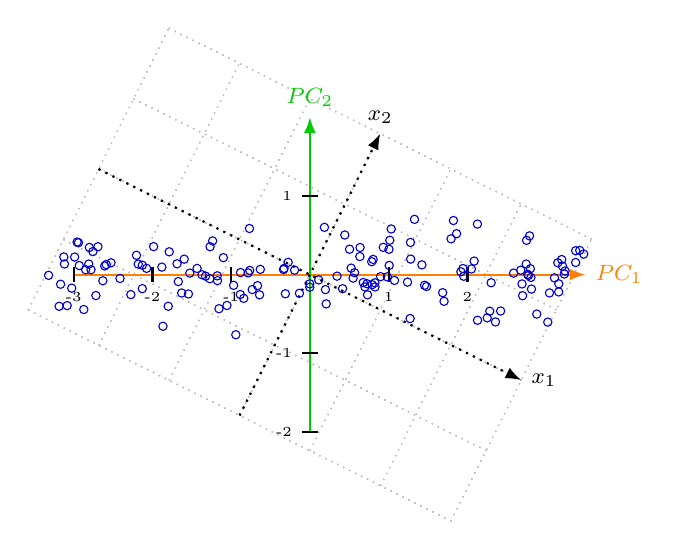
\begin{tikzpicture}
% Define the transformation matrix A_inv
\pgfmathsetmacro{\a}{0.894762}  %element (1,1) <--> (row,column)
\pgfmathsetmacro{\b}{0.446542}  %element (1,2)
\pgfmathsetmacro{\c}{-0.446542} %element (2,1)
\pgfmathsetmacro{\d}{0.894762}  %element(2,2)

    % Draw horizontal gridlines
    \foreach \y in {-2,-1,0,1,2} {
        \foreach \x in {-3,-2,...,3} {
            % Compute the transformed start and end points
            \pgfmathsetmacro{\xstart}{\a*(-3) + \b*\y}
            \pgfmathsetmacro{\ystart}{\c*(-3) + \d*\y}
            \pgfmathsetmacro{\xend}{\a*3 + \b*\y}
            \pgfmathsetmacro{\yend}{\c*3 + \d*\y}
            % Draw the transformed line
            \draw[gray!50, thin, dotted] (\xstart, \ystart) -- (\xend, \yend);
        }
    }

    % Draw vertical gridlines
    \foreach \x in {-3,-2,...,3} {
        \foreach \y in {-2,-1,0,1,2} {
            % Compute the transformed start and end points
            \pgfmathsetmacro{\xstart}{\a*\x + \b*(-2)}
            \pgfmathsetmacro{\ystart}{\c*\x + \d*(-2)}
            \pgfmathsetmacro{\xend}{\a*\x + \b*2}
            \pgfmathsetmacro{\yend}{\c*\x + \d*2}
            % Draw the transformed line
            \draw[gray!50, thin, dotted] (\xstart, \ystart) -- (\xend, \yend);
        }
    }

% X-axis with arrow and labeled ticks
\draw[thick, orange, -{Latex[length=2mm]}] (-3,0) -- (3.5,0) node[right] {{\footnotesize $PC_1$}};
\foreach \x in {-3,-2,-1,1,2}
  \draw[thick] (\x,0.1) -- (\x,-0.1) node[below] {{\tiny \x}};

% X-axis with arrow and labeled ticks
\draw[thick, dotted, -{Latex[length=2mm]}] (-3*0.894762,3*0.446542) -- (3*0.894762,3*-0.446542) node[right] {{\footnotesize $x_1$}};


% Y-axis with arrow and labeled ticks
\draw[thick, green!80!black, -{Latex[length=2mm]}] (0,-2) -- (0,2) node[above] {{\footnotesize $PC_2$}};
\foreach \y in {-2,-1,1}
  \draw[thick] (0.1,\y) -- (-0.1,\y) node[left] {{\tiny \y}};

\draw[thick, dotted, -{Latex[length=2mm]}] (-2*0.446542,-2*0.894762) -- (2*0.446542,2*0.894762) node[above] {{\footnotesize $x_2$}};


% Plot the ScatterPlot Data from PCA_FullExampleRotation_Data.txt
\foreach \x/\y in {
-1.2355/0.4279,
-0.2762/0.1559,
2.752/0.4354,
2.7894/0.492,
3.3754/0.1541,
-2.7178/-0.2661,
-1.0992/0.2155,
-2.6297/-0.078,
1.4223/0.1235,
-1.2699/-0.0522,
-3.0247/-0.1721,
3.1485/0.1507,
0.8271/-0.1563,
1.2778/0.4085,
2.5867/0.0189,
0.5486/-0.0447,
-1.3698/-0.0012,
1.7927/0.4544,
-0.8808/0.0261,
2.0857/0.172,
-3.1845/-0.4025,
3.4269/0.3072,
1.8226/0.6871,
2.7657/0.0036,
-1.5252/0.019,
3.1978/0.1912,
-3.1172/0.1349,
3.2401/0.0463,
-2.9567/0.4137,
-1.7867/0.2899,
-2.8715/-0.4431,
0.6371/0.3439,
-0.8843/-0.2526,
2.7015/-0.268,
2.6939/-0.1183,
-0.7323/-0.1899,
3.1608/-0.1171,
1.0323/0.5798,
-1.1737/-0.0759,
-1.1769/-0.0155,
1.0142/0.4365,
-2.0739/0.0795,
2.7757/-0.0114,
1.2396/-0.0952,
-2.9395/0.4053,
-0.133/-0.2368,
1.8629/0.5198,
-0.6395/-0.2569,
1.9535/-0.0209,
-2.1799/0.1336,
0.6776/-0.1,
2.7466/0.1343,
2.6778/0.056,
2.1288/-0.5797,
-2.6922/0.3543,
3.0209/-0.6036,
-1.3251/-0.0191,
3.106/-0.041,
2.8811/-0.5011,
1.0071/0.1163,
-2.8483/0.062,
-0.7679/0.5858,
-0.9689/-0.1359,
3.0426/-0.2325,
-2.6063/0.1098,
-1.4332/0.0781,
-2.801/0.3449,
0.8977/-0.0259,
3.2309/0.0075,
1.7037/-0.3393,
-3.1664/-0.1221,
-0.7842/0.0212,
-1.5966/0.1963,
1.0042/0.3218,
1.6862/-0.2294,
-2.1281/0.1194,
0.2068/-0.3716,
0.1843/0.6002,
-2.2023/0.2456,
-0.6651/-0.1402,
2.8065/-0.0361,
-1.6711/-0.0885,
2.252/-0.5492,
-0.8401/-0.3016,
0.8255/-0.1043,
-1.0534/-0.3918,
0.1972/-0.1904,
0.7895/-0.1276,
-1.9845/0.3555,
2.3569/-0.6006,
3.4776/0.261,
0.4151/-0.1787,
0.5244/0.0823,
0.5033/0.3225,
1.3282/0.7019,
-2.7799/0.0619,
0.9316/0.3463,
2.2836/-0.4648,
-2.9292/0.115,
1.9433/0.0771,
3.1595/-0.2195,
1.2796/0.1971,
-1.6289/-0.2333,
-2.4118/-0.0489,
2.3018/-0.1031,
-0.0016/-0.1172,
-0.6297/0.0668,
2.4218/-0.4623,
-1.6874/0.1373,
1.9172/0.0361,
1.4557/-0.1353,
0.7319/-0.2566,
0.443/0.5033,
-0.3284/0.0789,
-2.5257/0.1503,
-2.587/0.1272,
-1.1545/-0.4328,
0.7847/0.1641,
0.567/0.0241,
-1.8803/0.0952,
-2.7563/0.2924,
2.0511/0.0716,
0.8029/0.1929,
2.8138/-0.1839,
-3.319/-0.009,
-1.543/-0.2458,
3.375/0.3031,
1.2726/-0.5577,
0.7252/-0.116,
0.9825/-0.0283,
-3.1256/0.2241,
-3.0828/-0.3934,
1.0743/-0.0738,
-2.8088/0.1343,
-1.2674/0.3549,
0.6346/0.2296,
1.4813/-0.1507,
2.1273/0.6417,
-0.7641/0.0536,
-0.3348/0.064,
2.7993/0.0751,
-2.1285/-0.1782,
-1.8662/-0.6558,
0.6991/-0.1559,
-1.7993/-0.402,
-2.9881/0.223,
-0.9409/-0.7635,
0.3444/-0.0198,
3.2087/0.1077,
-2.2742/-0.2536,
-0.1951/0.0569,
-0.3116/-0.2436,
0.1117/-0.0672,
-0.0017/-0.1602
} 
{
% Draw horizontal line to x-axis
%\draw[red!70!black, dotted, thick] (\x,0) -- (\x,\y);

% Draw the point
\draw[blue!80!black] (\x,\y) circle (1.5pt);
}

\end{tikzpicture}
\end{document}
